\chapter{提案手法}\label{chap:method}
本章では,従来手法をベースとする提案手法を
提案手法の概要,提案手法における学習フェーズ,テストフェーズと用いた目標方向について
の4節に分けて述べる.

\section{提案手法の概要}

% 1章の背景で述べた分岐路において,ルートを選択する場合に
% 入力する情報としてカメラ画像のみでは「右と左のどちらに曲がる」という判断をするための
% 情報が不足していると考えられる.
従来手法で用いたデータセットと学習器の入力へ,
「直進」「左折」などの目標方向指令を追加することで,
学習器の出力による走行において,経路を選択する機能の追加を行った.
なお,追加した要素以外は従来手法と同様である.
% 本研究で対象とするロボットの構造,搭載するセンサを\ref{fig::turtlebot3_gazo}とし,

% 提案手法の概要をFig.\ref{fig::method_abs}

% \begin{figure}[H]
%     \centering
%     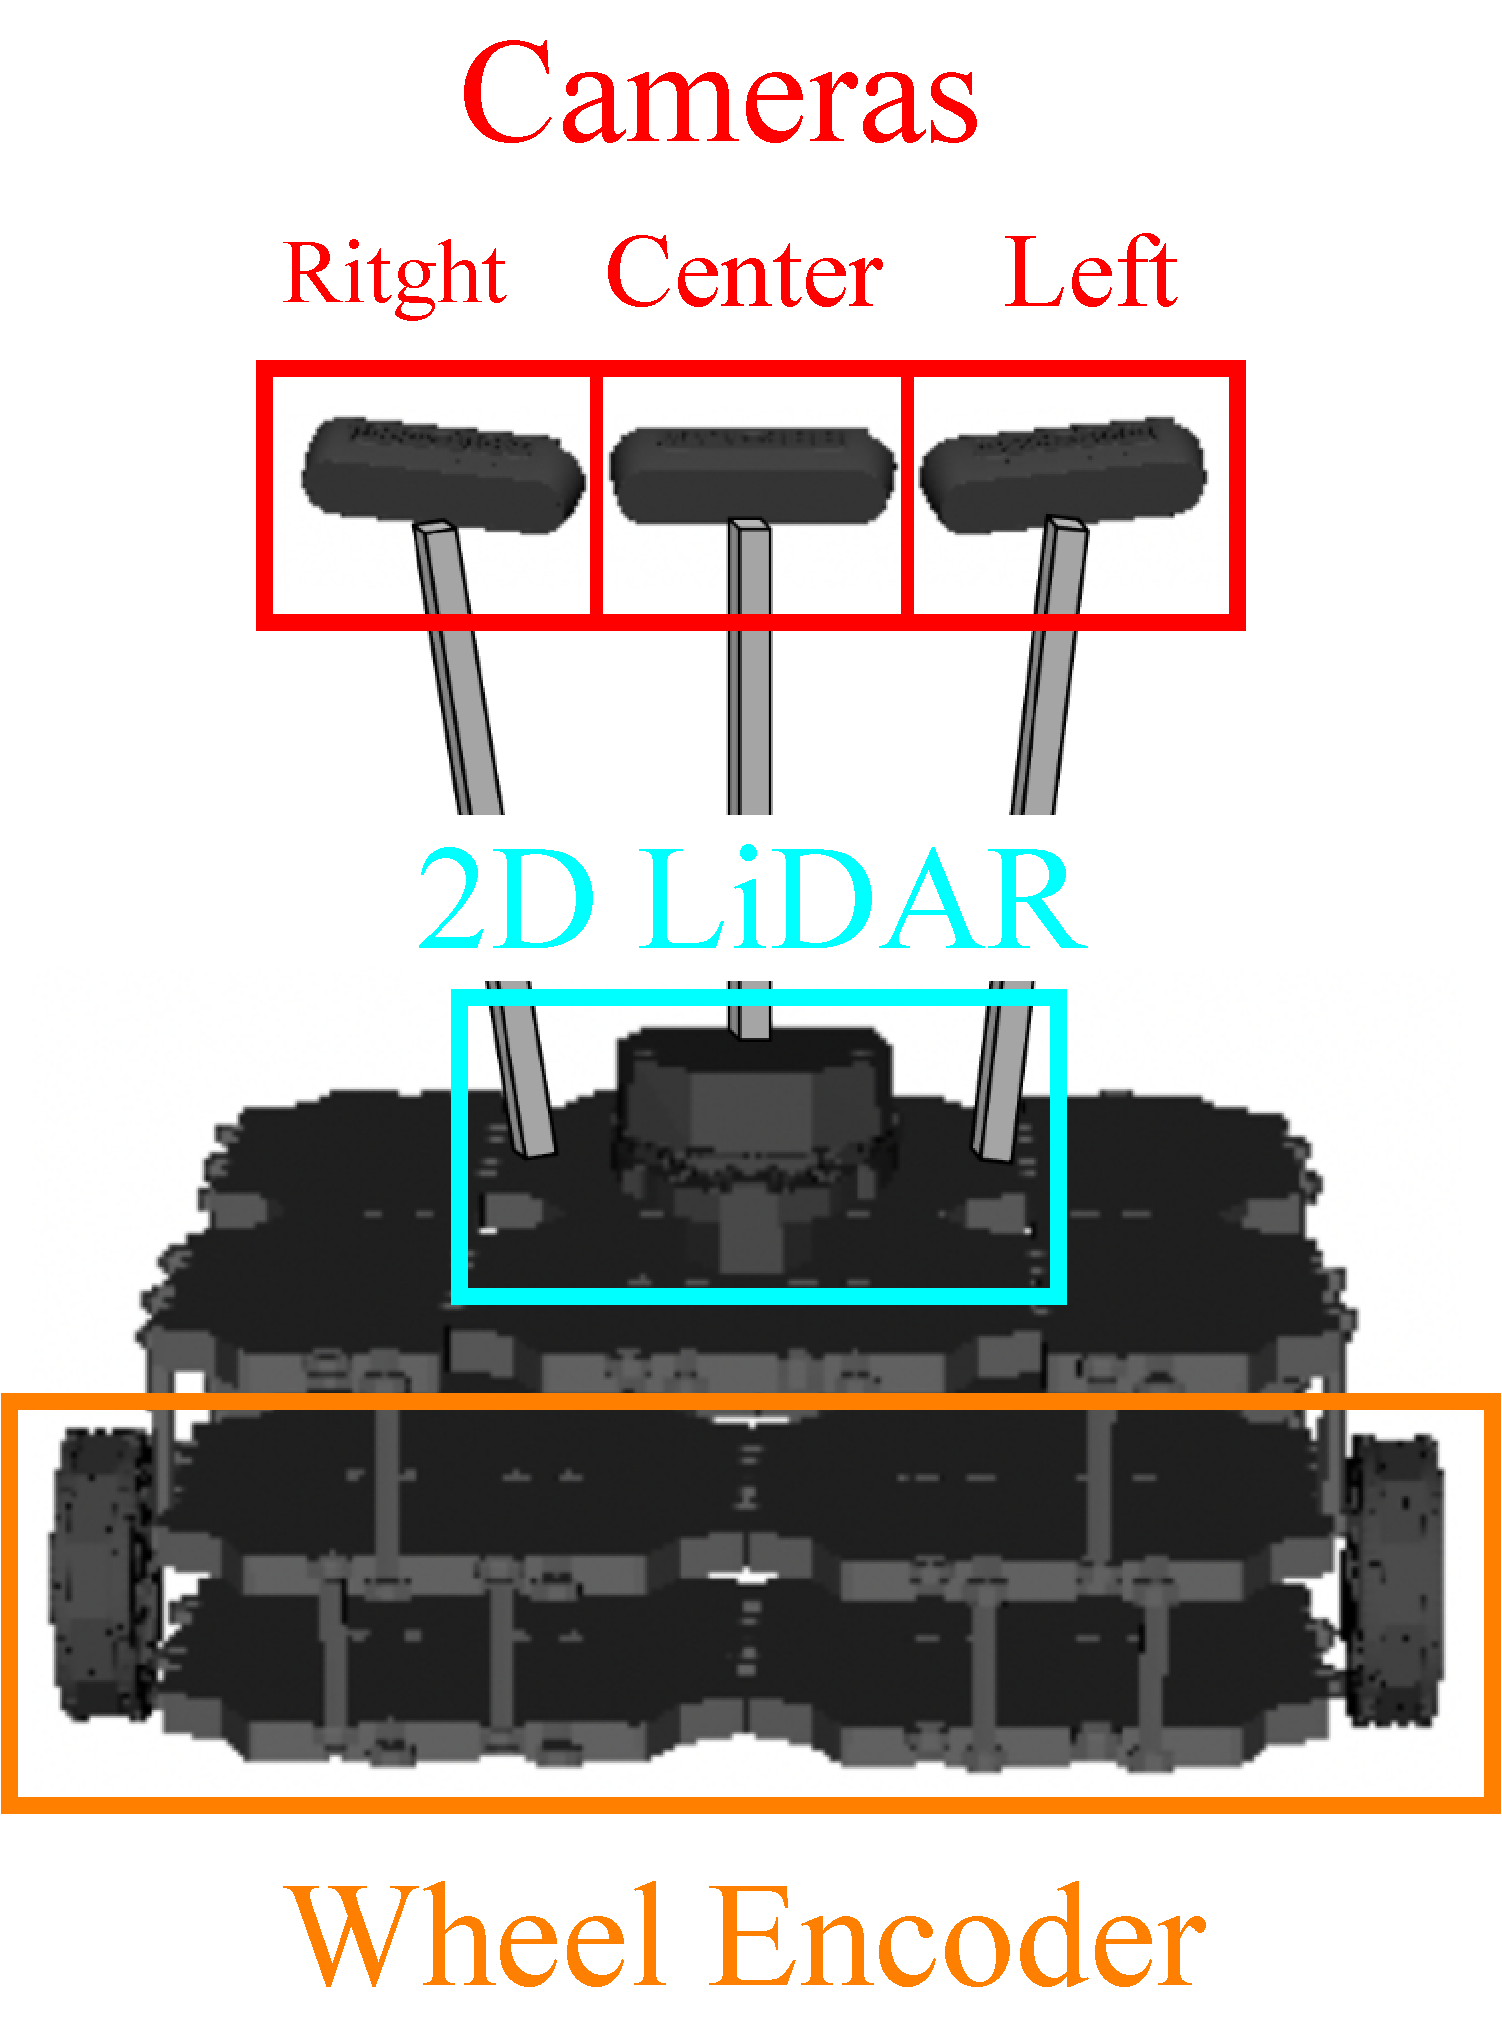
\includegraphics[width = 4cm]{./figs/turtlebot3_kame.pdf}
%     \caption{turtlebot3 waffle}
%     \label{fig::turtlebot3_gazo}
% \end{figure}

% \begin{figure}[H]
%     \begin{tabular}{c}
%       \begin{minipage}[t]{0.5\hsize}
%         \centering
%         % \vspace{-1.0zh}
%         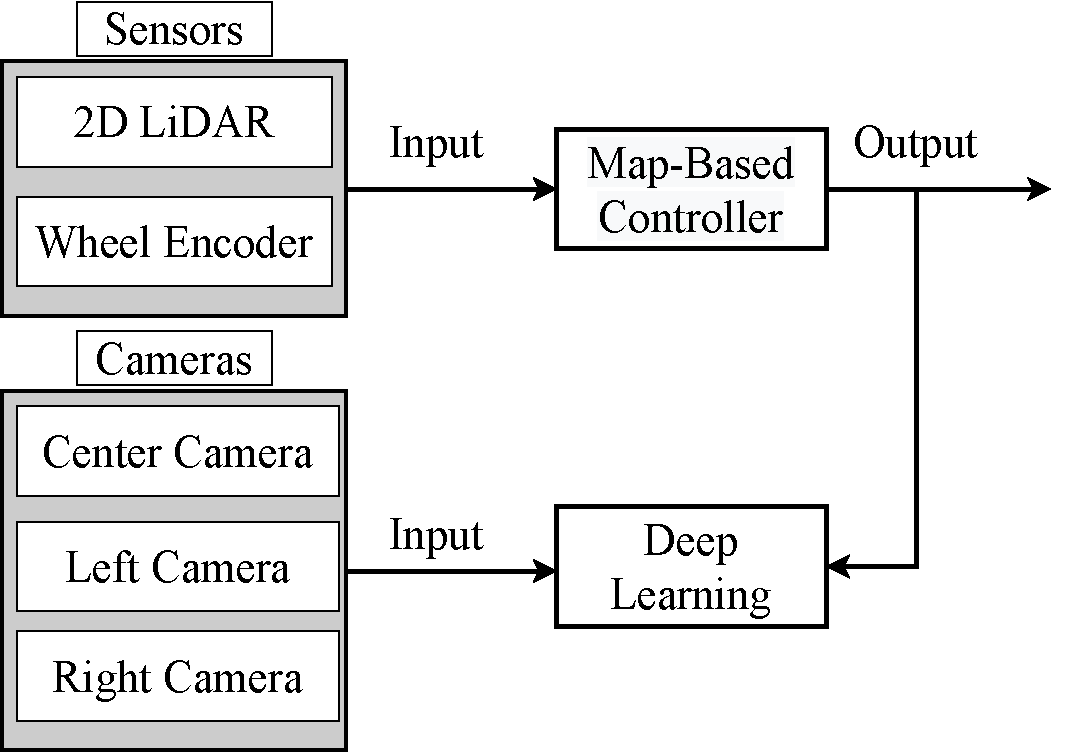
\includegraphics[keepaspectratio, scale=0.35]{./figs/system_abs.pdf}
%         \subcaption{Learning phase}
%         \label{fig::learning_abs}
%       \end{minipage}
%       \begin{minipage}[t]{0.5\hsize}
%         \centering
        
%         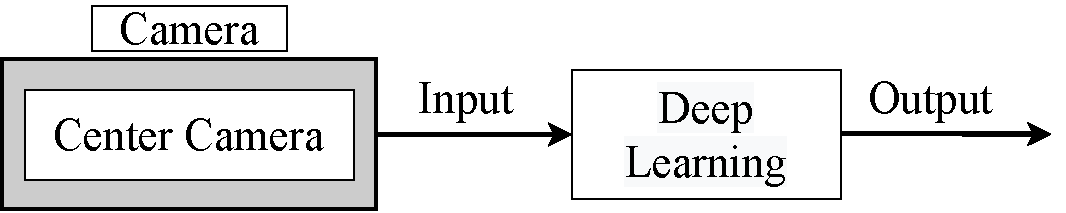
\includegraphics[keepaspectratio, scale=0.35]{./figs/system_test_abs.pdf}
%         \subcaption{Test phase}
%         \label{fig::test_abs}
%       \end{minipage}
%       \vspace{2.0zh}
%     \end{tabular}
%      \caption{Concept of the proposed method}
%      \label{fig::method_abs}
%   \end{figure} 


    
    % \begin{table}[h]
    %   \centering
    %   \caption{Target Direction list}
    %   \begin{tabular}{ccccll}
    %   \cline{1-5}
    %   \multicolumn{1}{|c|}{Target Direction} & \multicolumn{1}{c|}{continue}&\multicolumn{1}{c|}{go straight}          & \multicolumn{1}{c|}{turn left}          & \multicolumn{1}{c|}{turn right}          &  \\ \cline{1-5}
    %   \multicolumn{1}{|c|}{Data}  &\multicolumn{1}{c|}{{[}100, 0, 0, 0{]}}& \multicolumn{1}{c|}{{[}0, 100, 0, 0{]}} & \multicolumn{1}{c|}{{[}0,0,100, 0{]}} & \multicolumn{1}{l|}{{[}0, 0, 0, 100{]}} &  \\ \cline{1-5}
    %                              &                                  &                                  &                                  &  \\
    %                              &                                  &                                  &                                  &  \\
    %   \multicolumn{1}{l}{}       &                                  &                                  &                                  & 
    %   \end{tabular}
    %   \vspace{-3.0zh}
    %   \label{tb:command_4}
    %   \end{table}

\newpage
\section{学習フェーズ}
\label{lerning}
学習器の訓練を行う学習フェーズで用いるシステムをFig. \ref{fig::learningsystem}示す.
経路追従行動を行う地図べースの制御器へ目標方向の生成機能と,データセットへ目標方向の追加を行った.
提案手法では,\ref{fig::learning_abs}に示すように
LiDARとオドメトリを入力とする地図べースの制御器による経路追従行動を,
カメラ画像と目標方向を用いて模倣学習する.
  \begin{figure}[h]
    \centering
    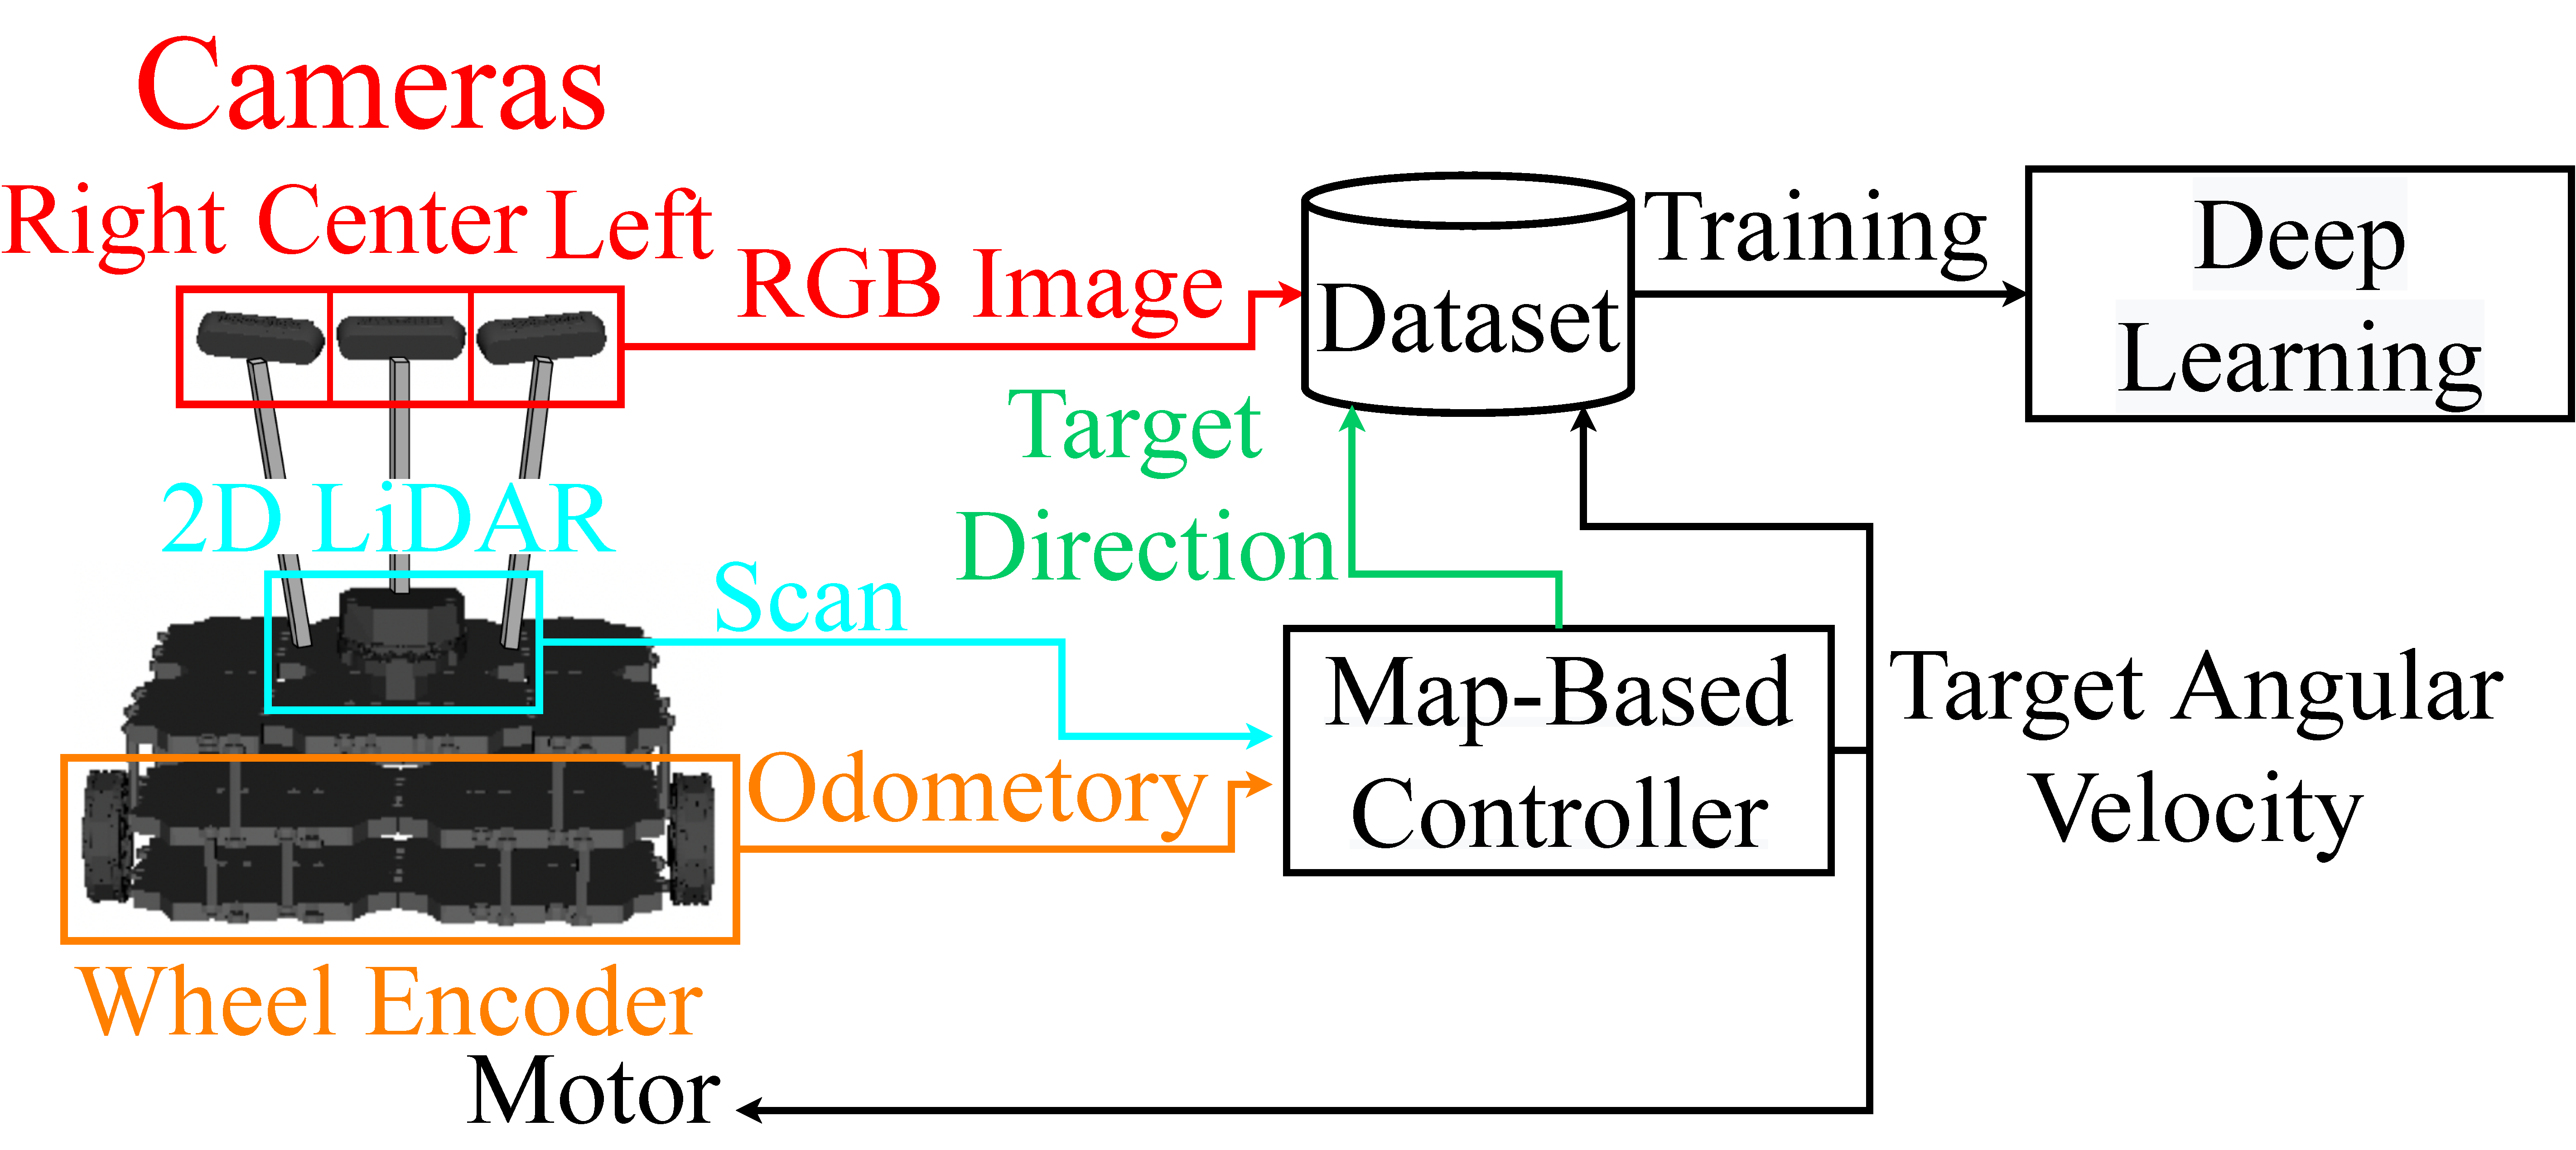
\includegraphics[width = 12cm]{./figs/system_learning.pdf}
    \caption{Learning phase of proposed method}
    \label{fig::learningsystem}
\end{figure}
\begin{figure}[h]
  \centering
  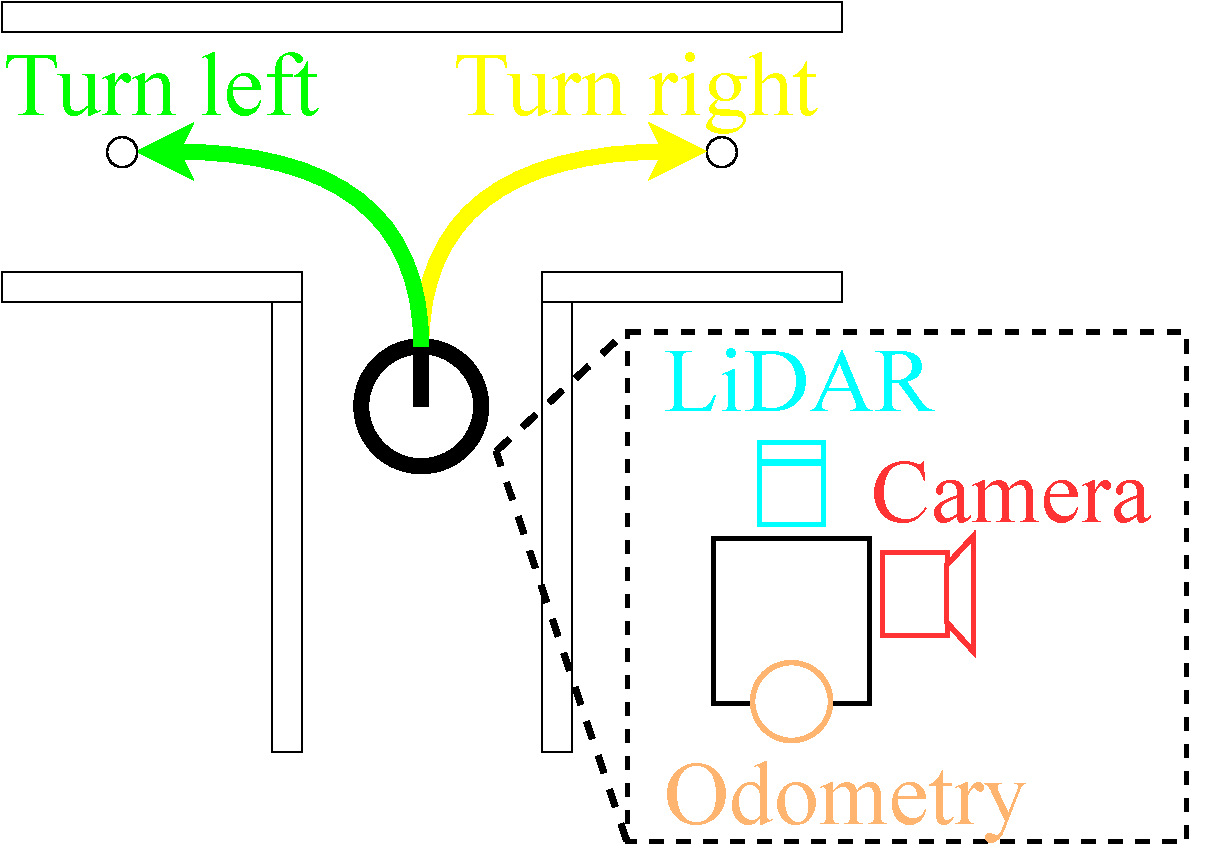
\includegraphics[width = 9.5cm]{./figs/ler_abs.pdf}
  \caption{Overview learning phase}
  \label{fig::learning_abs}
\end{figure}
\newpage
\section{テストフェーズ}
\label{test}
提案手法におけるテストフェーズではFig. \ref{fig::testsystem}で示すように,
学習器の入力へ目標方向を追加した.
\ref{fig::test_abs}に動作の様子を示す.
カメラ画像と目標方向を用いた学習器の
出力による走行において,目標方向によって経路の選択を行う.
% 地図ベースの制御器の出力による動作から,中央のカメラ画像と目標方向を入力とした
% 学習器の出力による動作へ切り替えて走行を行う.
% テスト時の目標方向の生成(方向の指示)はJoy\_stickコントローラのボタンを用いて行う.
% また,目標方向は学習フェーズと同じ形式,データを用いる.
% テストフェーズにおける手順を下記に示す.
% \begin{enumerate}
%     \item 機体に取り付けた中央のカメラからRGB画像,Joy\_stickコントローラより目標方向のデータを取得
%     \item 取得したデータ(カメラ画像,目標方向)を学習器へ入力
%     \item 学習器の出力である角速度をモータへ与える
%   \end{enumerate}


\begin{figure}[h]
    \centering
    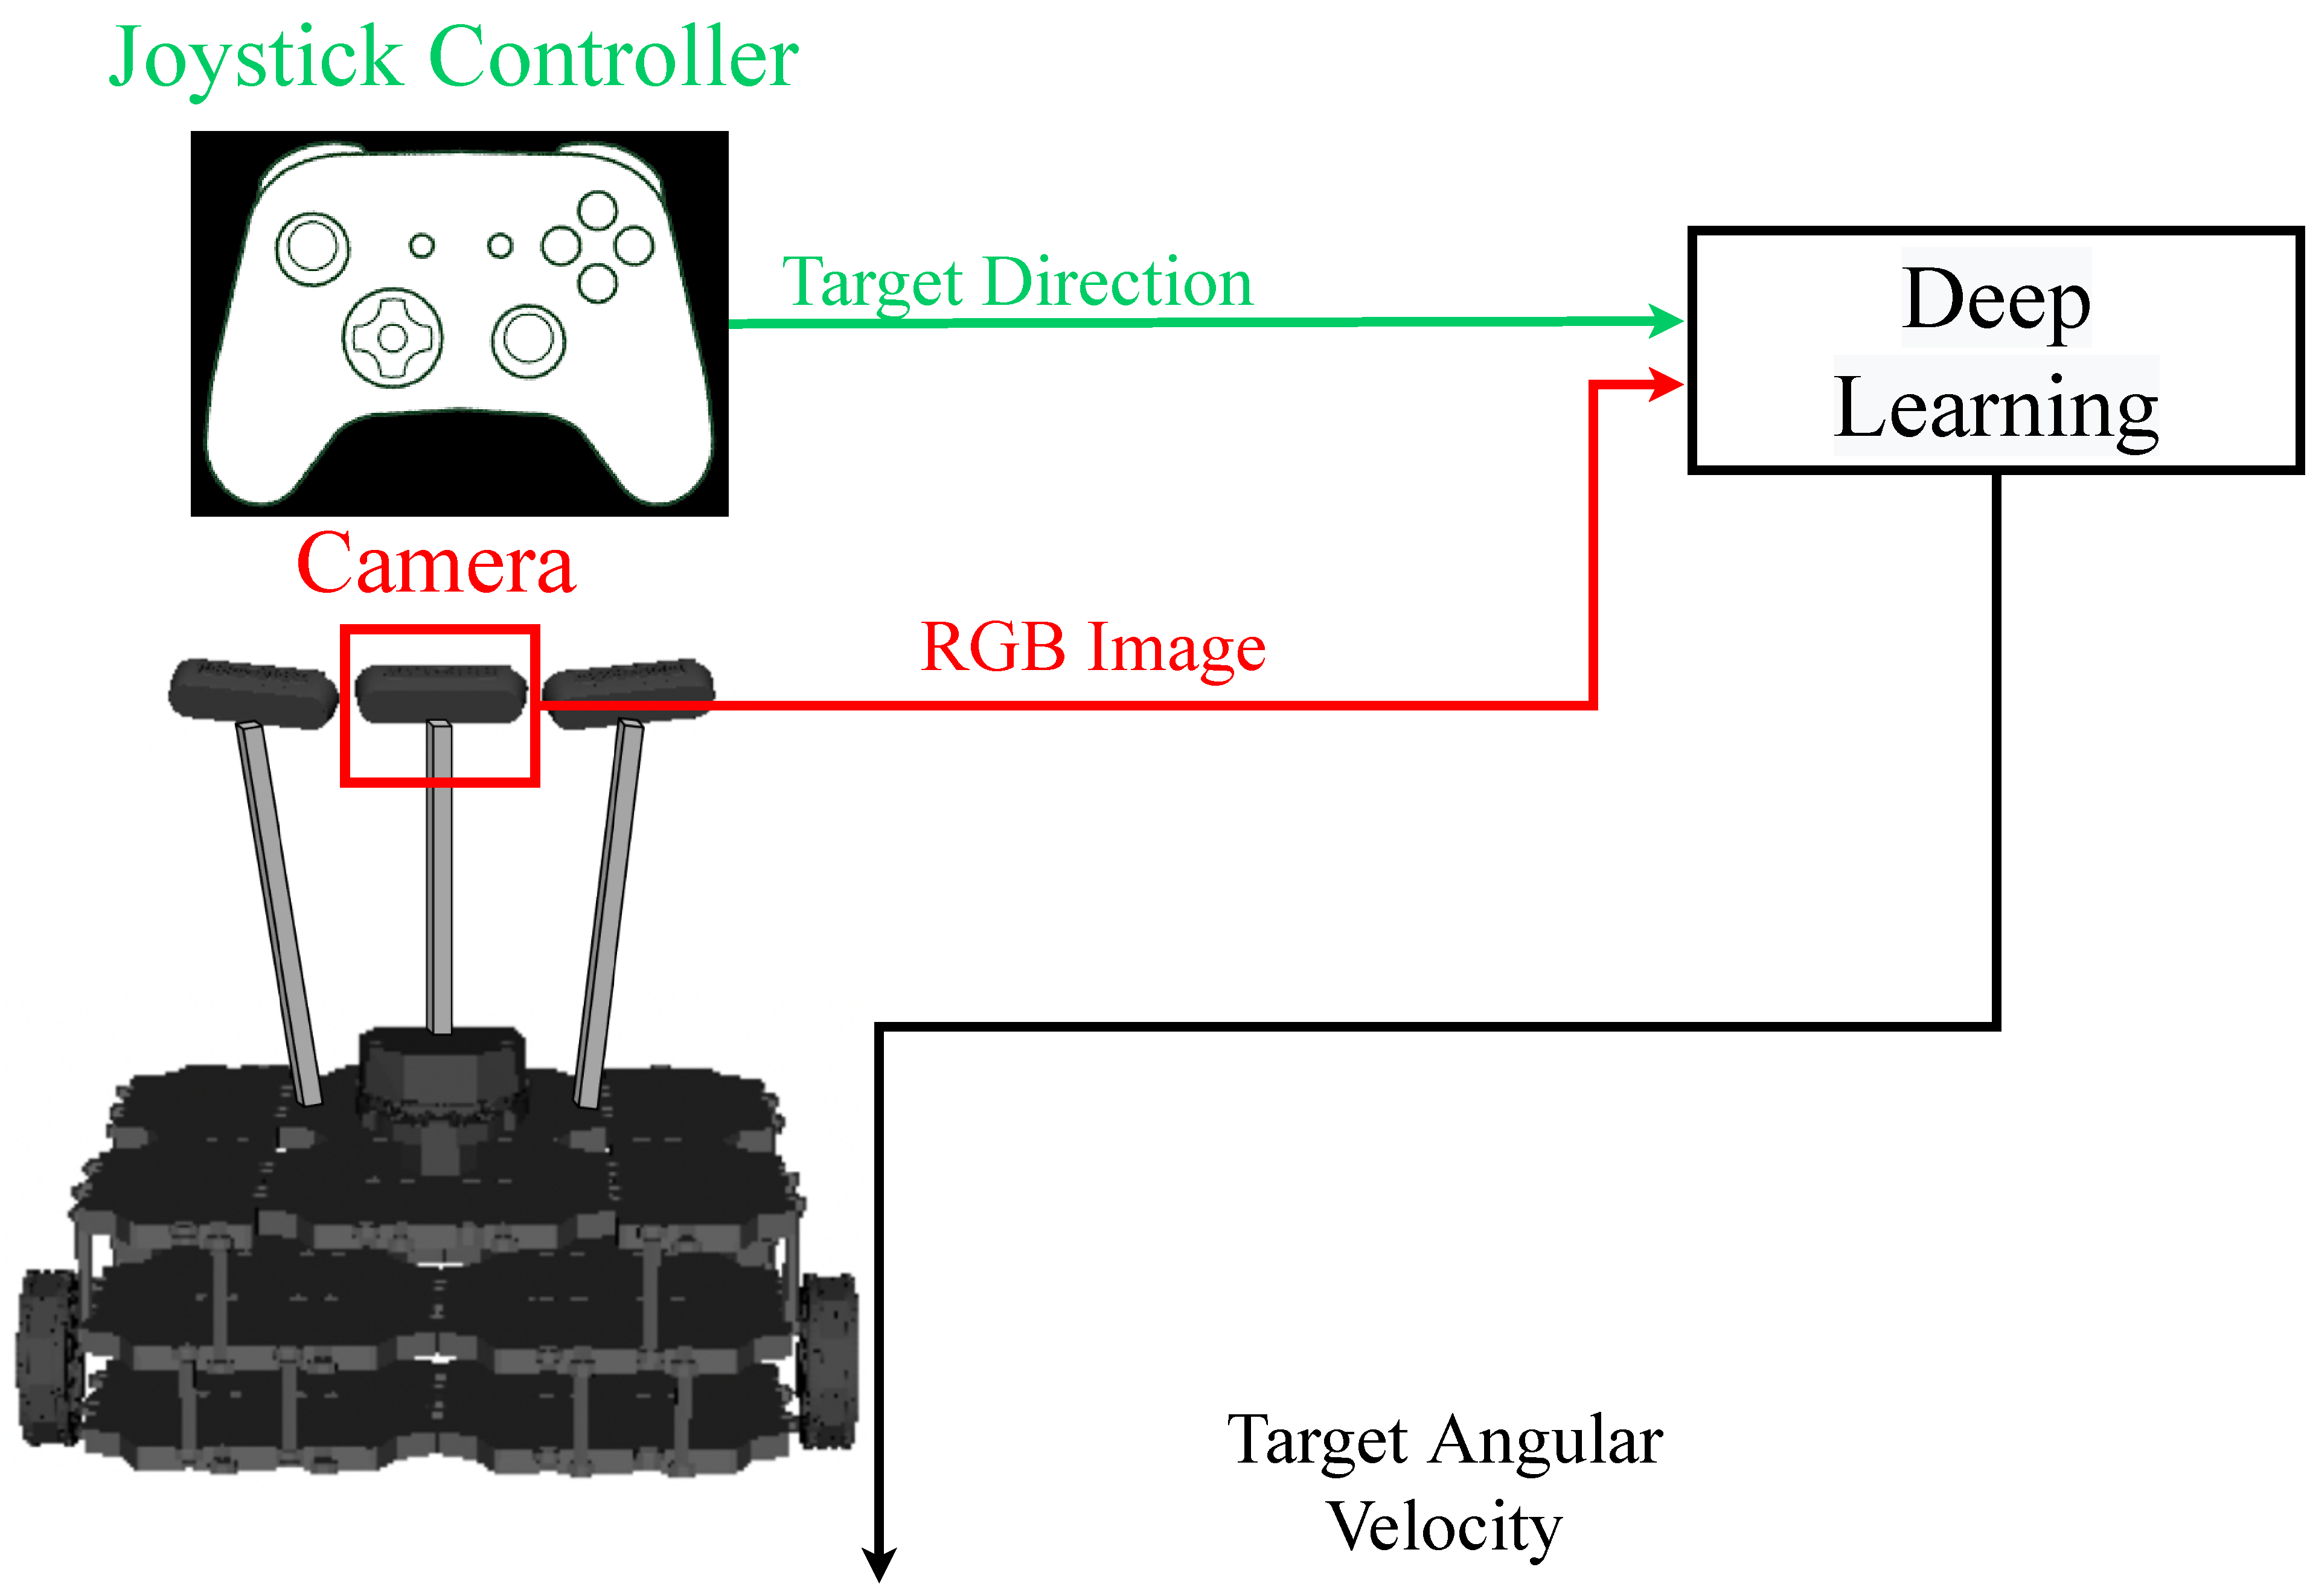
\includegraphics[width = 9cm]{./figs/system_test.pdf}
    \caption{Test phase of proposed method}
    \label{fig::testsystem}
\end{figure}
\begin{figure}[h]
  \centering
  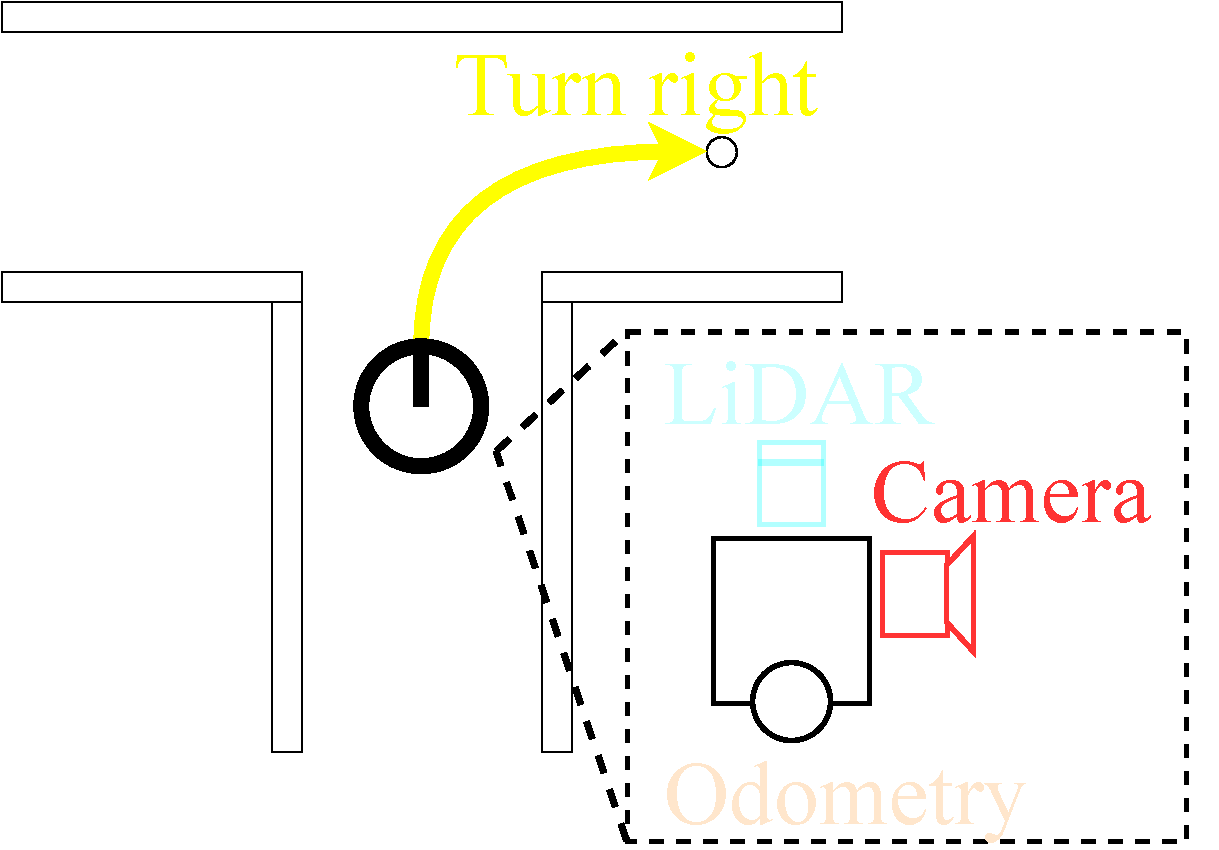
\includegraphics[width = 9cm]{./figs/test_abs.pdf}
  \caption{Overview test phase}
  \label{fig::test_abs}
\end{figure}

\newpage
\section{目標方向}
本研究で用いた目標方向と,そのデータ形式である目標方向指令について述べる.
目標方向はFig.\ref{fig::cmd_4}に示す.
経路を「道なり」に走行(Continue)
分岐路において「直進(Go straight)「左折(Turn left)」「右折(Turn right)」の4つとする,
\begin{figure}[h]
  \centering
  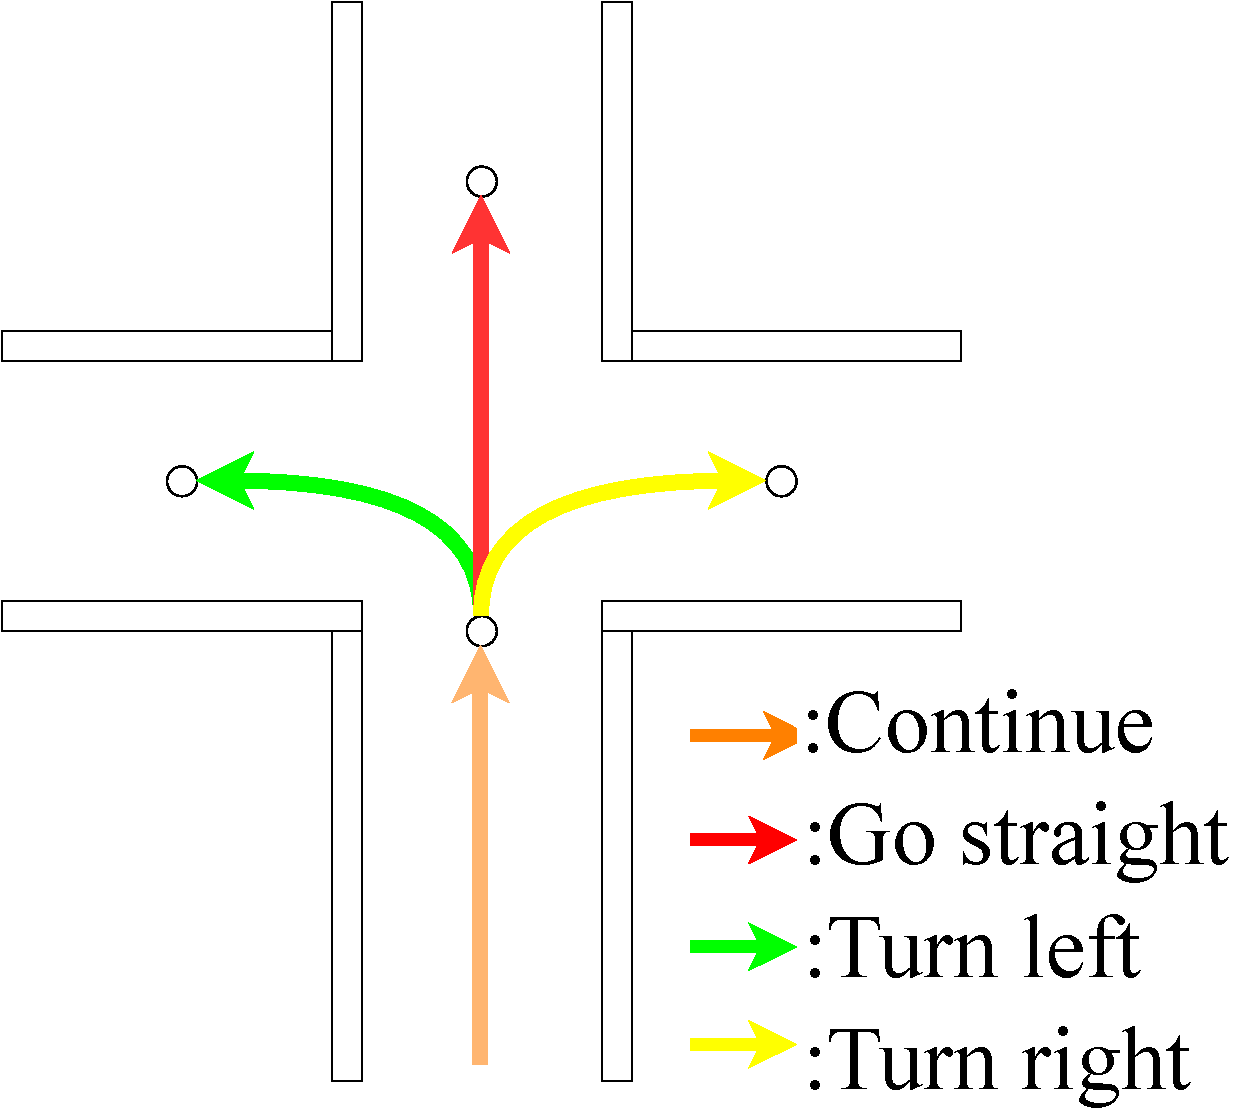
\includegraphics[width = 9.5cm]{./figs/cmd_4.pdf}
  \caption{Target direction}
  \label{fig::cmd_4}
\end{figure}

学習器には,上記の4つの目標方向を,要素数4,次元数1のint型の
配列(One-Hot ベクトル)で表現した”目標方向指令”を入力する.
目標方向指令のデータ形式をTable \ref{tb:command_4}に示す.
  %   \begin{table}[h]
  %     \caption{Target direction and data}
  %     \label{tb:command_4}
  %     \begin{center}
  %         \vskip 0.5zh
  %         \begin{tabular}{|c|c|}
  %             \hline
  %             Target direction & Data\\ \hline
  %             Continue & $[100, 0, 0, 0]$ \\ \hline
  %             Go straight & $[0, 100, 0, 0]$ \\ \hline
  %             Turn left& $[0, 0, 100, 0]$ \\ \hline
  %             Turn right & $[0, 0, 0, 100]$ \\ \hline
  %         \end{tabular}
  %     \end{center}
  % \end{table}

 \begin{table}[h]
      \centering
      \caption{Target direction list}
      \begin{tabular}{ccccll}
      \cline{1-5}
      \multicolumn{1}{|c|}{Target Direction} & \multicolumn{1}{c|}{Continue}&\multicolumn{1}{c|}{Go straight}          & \multicolumn{1}{c|}{Turn left}          & \multicolumn{1}{c|}{Turn right}          &  \\ \cline{1-5}
      \multicolumn{1}{|c|}{Data}  &\multicolumn{1}{c|}{{[}100, 0, 0, 0{]}}& \multicolumn{1}{c|}{{[}0, 100, 0, 0{]}} & \multicolumn{1}{c|}{{[}0, 0, 100, 0{]}} & \multicolumn{1}{l|}{{[}0, 0, 0, 100{]}} &  \\ \cline{1-5}
                                 &                                  &                                  &                                  &  \\
                                 &                                  &                                  &                                  &  \\
      \multicolumn{1}{l}{}       &                                  &                                  &                                  & 
      \end{tabular}
      \vspace{-3.0zh}
      \label{tb:command_4}
      \end{table}
\newpage
\section{ネットワーク構造}
\label{net}
今回の提案手法で用いた,カメラ画像と目標方向を入力とする学習器の
ネットワークをFig. \ref{fig::methodnetwork}に示す.
また,ハイパーパラメータについてTable \ref{tb::param}に示す.
64×48のRGB画像を入力とする入力層1,畳込み層3,全結合層2層を持つ6層のCNNと,CNNの出力と目標方向指令を入力する入力層1,
全結合層2.出力層1の全10層の構造になっている.
出力はヨー方向の角速度である.

\begin{figure}[h]
    \centering
    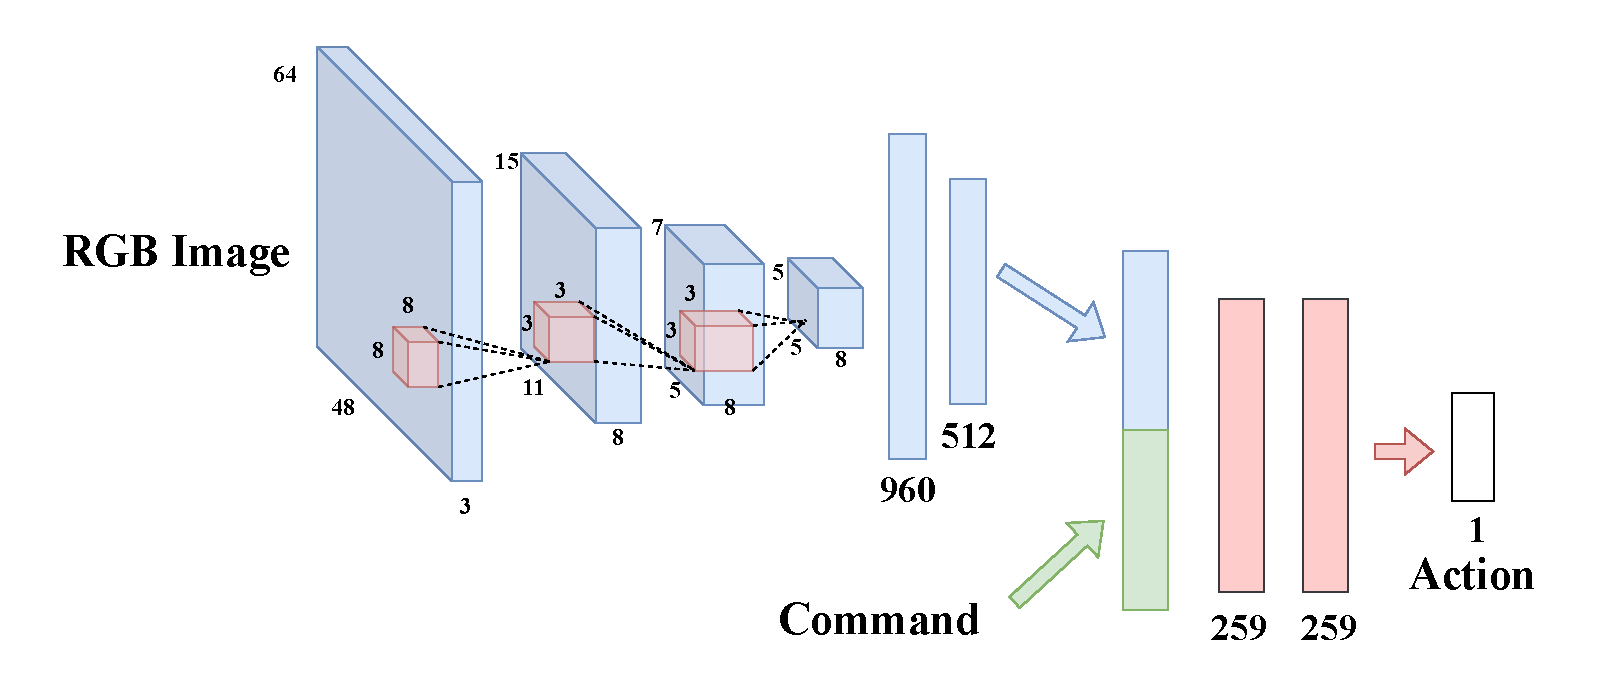
\includegraphics[width = 13cm]{./figs/network.pdf}
    \caption{Method network}
    \label{fig::methodnetwork}
\end{figure}
% \vspace{-1.0zh}
\begin{table}[htb]
    \centering
    \caption{Parameters of deep learning}
    \begin{tabular}{|c|c|c|c|}
    \hline
    Input data    & Image (64x48 pixels, RGB channels) , Target direction                                             \\ \hline
    Optimizer     & Adam ($alpha = 0.001, beta1 = 0.9, beta2 = 0.999, eps = 1e^{-1}$ )  \\ \hline
    Loss function & Softmax-cross-entropy                                                            \\ \hline
    Output data   & Angular velocity                                              \\ \hline
    \end{tabular}
    \label{tb::param}
    \end{table}





